%!TEX root = ../main.tex

\chapter{Perceived valence}
\label{ch:4}

In the study presented in Chapter \ref{ch:3}, we didn't manage to identify behavioural differences when comparing tracks which have been previously reported as being able to cause MECs with tracks which were matched to those by artist, duration, and popularity. We hypothesised that this might have been due to small effect sizes, not detectable in behavioural experiments with relatively small sample sizes, and that applying computational methods to larger amounts of data might have the potential to identify differences between these two sets of tracks. 

This chapter presents the application of such methods to the investigation of the relationship between valence on MECs. More specifically, since valence is a readily available feature for computational analysis, as explained below, it was chosen as a proof of concept to justify further computational work, as presented in Chapter \ref{ch:5}. With this study, we aimed to disentangle findings that MECs have been linked to both happiness and sadness expressed by music. We conducted a computational analysis on a corpus of 988 tracks previously reported to elicit MECs, by comparing them with a control set of tracks matched by artist, duration, and popularity, hereafter referred to as tracks from the matched source. We analysed track-level audio features obtained with the Spotify Web API\footnote{\url{https://developer.spotify.com/documentation/web-api}} across the two sets of tracks, resulting in confirmatory findings that tracks which cause MECs were sadder than tracks from the matched source, and exploratory findings that they were also slower, less intense, and more instrumental than tracks from the matched source on average. We also found that the audio characteristics of tracks from the chills source were related to the direction and magnitude of the difference in valence between the two sets of tracks. We discuss these results in light of the current literature on valence and MECs in music, provide a new interpretation in terms of personality correlates of musical preference, and review the advantages and limitations of our computational approach.

\section{Introduction}
\label{se:val-intro}

As discussed in Chapter \ref{ch:2}, particular attention has been given to elicitors of MECs, resulting in the identification of a range of acoustic and musical features usually associated with the experience of MECs, such as sudden dynamic changes, increased roughness, crescendi, or the entrance of new instruments. These features represent local musical and auditory events, and are therefore reflective of the fleeting nature of MECs.

In contrast to continuous changes within musical stimuli, emotional characteristics of entire musical pieces have also been investigated. As a result, MECs have been associated with perceived valence. However, there is disagreement about the direction of this relationship. While \textcite{grewe2011} reported an increase in frequency of MECs for positively valenced music, \textcite{panksepp1995} found that MECs were more frequently associated with perceived sadness. In the latter study, however, both happy and sad music were found to elicit MECs, reflecting subsequent findings that MECs are associated with both emotions when they are expressed by music \parencite{bannister2020a, mori2017, panksepp1995}.

Conflicting effects of valence on MECs have been discussed in the context of being moved, a mixed emotional state involving sadness and joy \parencite{menninghaus2015}. More specifically, being moved has been associated with MECs when listening to music \parencite{bannister2019, bannister2020a, bannister2018, benedek2011}, and has been found to mediate the relationship between liking and sadness in response to music \parencite{vuoskoski2017}. Moving stimuli often feature narrative displays of social separation or reunion \parencite{wassiliwizky2015}, prosocial behaviour \parencite{wassiliwizky2017a}, or self-sacrifice \parencite{konecni2007b}, but it remains unclear how such narrative features translate to music, and how stimulus valence relates to the occurrence of MECs. It could be that sad music provides an emotional context more conducive to the occurrence of MECs \parencite{panksepp1995}. Another plausible explanation for the mixed effects of valence on MECs comes from the possibility that MECs encompass several phenomenologically distinct experiences, partly characterised by different degrees of felt emotions \parencite{bannister2019, maruskin2012}.

This perspective was further developed in Chapter \ref{ch:2}, in which a preliminary model suggests three different pathways for the experience of MECs, linking different types of elicitors to the combination of psychological and evolutionary mechanisms most likely to elicit MECs, if not different types of MECs. In one such pathway, individuals with high trait empathy are suggested to be more receptive to emotional elicitors of MECs, such as perceived valence, leading them to mimic the perceived emotion through a process called emotional contagion, and then to experience MECs through the process of being moved. Other pathways link acoustic and musical elicitors to processes involving arousal and musical expectation, respectively. There is little research on the existence of these pathways, and confirming or refuting an effect of perceived valence on MECs would be a useful step in providing support for the existence of one of them, leading to a better understanding of the causes of MECs, and in turn, of music appreciation in general.

In light of the current evidence, it remains difficult to establish the role of expressed stimulus valence on the incidence of MECs. While behavioural approaches have contributed to identifying conflicting effects of happiness and sadness, they remain limited due to the number of stimuli which can be reasonably presented to participants, ranging here from 3 \parencite{bannister2018} to 23 \parencite{grewe2011}. Computational methods, however, can overcome such restrictions, and are well suited to the study of a large collection of naturalistic stimuli, at the cost of reduced control over experimental conditions. When we ran this study, there had been, to our knowledge, no use of corpus-based analysis in research on MECs, despite the success of similar approaches in research on music and emotion \parencite[e.g.,][]{eerola2011}. The analysis presented in this chapter was an attempt at addressing this gap in the literature, focusing on the effects of valence and other track-level audio features (i.e., features computed over entire musical pieces) on MECs.

Specifically, we compared features between tracks known to elicit MECs and a control set of tracks matched by artist, duration, and popularity. This experiment allowed us to collect large amounts of data. As a consequence, to promote transparency, we decided to clearly distinguish between confirmatory and exploratory analyses, as recommended by \textcite{dushoff2019}. First, we conducted confirmatory analyses regarding the effect of the valence feature on MECs, hypothesising a difference in expressed valence between the two sets of tracks. Then, we conducted two exploratory analyses, to investigate the influence of other features on the occurrence of MECs, and to assess whether these features influenced the direction and magnitude of the difference in valence between both sets of tracks, with the aim to reveal whether or not differences in musical characteristics (i.e., different types of music) could be the reason behind conflicting effects of valence on MECs. We discuss these results and the advantages and limitations of our approach, and provide a new interpretation with reference to a theory of the personality correlates of musical preference \parencite{rentfrow2011} introduced in Chapter \ref{ch:3}, identifying relationships between MECs and several dimensions capturing musical preference for \emph{sophisticated} music and \emph{intense} music.

\section{Methods}
\label{se:val-methods}

\subsection{Stimuli and features}

\subsubsection{Dataset}

For this study, we used \emph{ChiM},\footnote{ChiM version 1.0.0, available on Zenodo as a permanent archive, at \url{https://doi.org/10.5281/zenodo.3950516}} a dataset prepared by compiling every mention of a piece of music reported to elicit MECs in the literature reviewed in Chapter \ref{ch:2}, following the methods described below.

In ChiM, pieces of music were only included if they were confirmed to elicit MECs in at least one listener. As a result, some pieces of music mentioned in the literature were intentionally omitted, if occurrences of MECs were not precisely assigned to individual pieces of music \parencite[e.g.,][]{masherrero2014}, if no occurrences of MECs were recorded for specific pieces of music \parencite[e.g.,][]{grewe2007}, or if MECs occurred in response to stimuli combining music and other modalities \parencite[e.g.,][]{strick2015}. In the literature reviewed in Chapter \ref{ch:2}, most mentions of pieces of music were included directly in the text or in the associated supplementary materials. For \textcite{bannister2018}, data from the associated dataset \parencite{bannister2017} was also included.

The pieces of music were categorised according to whether each specific mention represented an anecdote by the authors, a participant report of MECs, an empirical verification of MECs, or a discussion of prior results. Artist names and song titles were harmonised across publications, most often following a basic search on Google or Wikipedia. Each mention of a piece of music was assigned a unique ID, and individual pieces of music were also assigned a unique ID in order to easily identify the ones which were mentioned several times in the literature, as indicated by an additional variable. Mentions of several movements from the same piece of music and otherwise duplicated mentions of pieces of music in the same publication were consolidated into a row with a single mention ID. Different performances or covers of a piece of music were assigned to the original composer, with a separate variable containing notes about further details on the performance. These pieces of music were assigned the same song ID with a distinct suffix. Finally, whenever a reasonable guess was possible, missing artist information was added. In other cases, missing information was indicated as such.

Version 1.0.0 of ChiM includes 988 mentions of music confirmed to induce MECs in at least one listener, which represents a much larger sample of music than the one explored in Chapter \ref{ch:3}, and was therefore well-suited for computational analysis. As seen in \autoref{fig:val-1}, the vast majority of ChiM consists of contributions from a few individual articles, and we can observe a slight over-representation of specific composers and pieces of music.

\begin{figure}[t!]
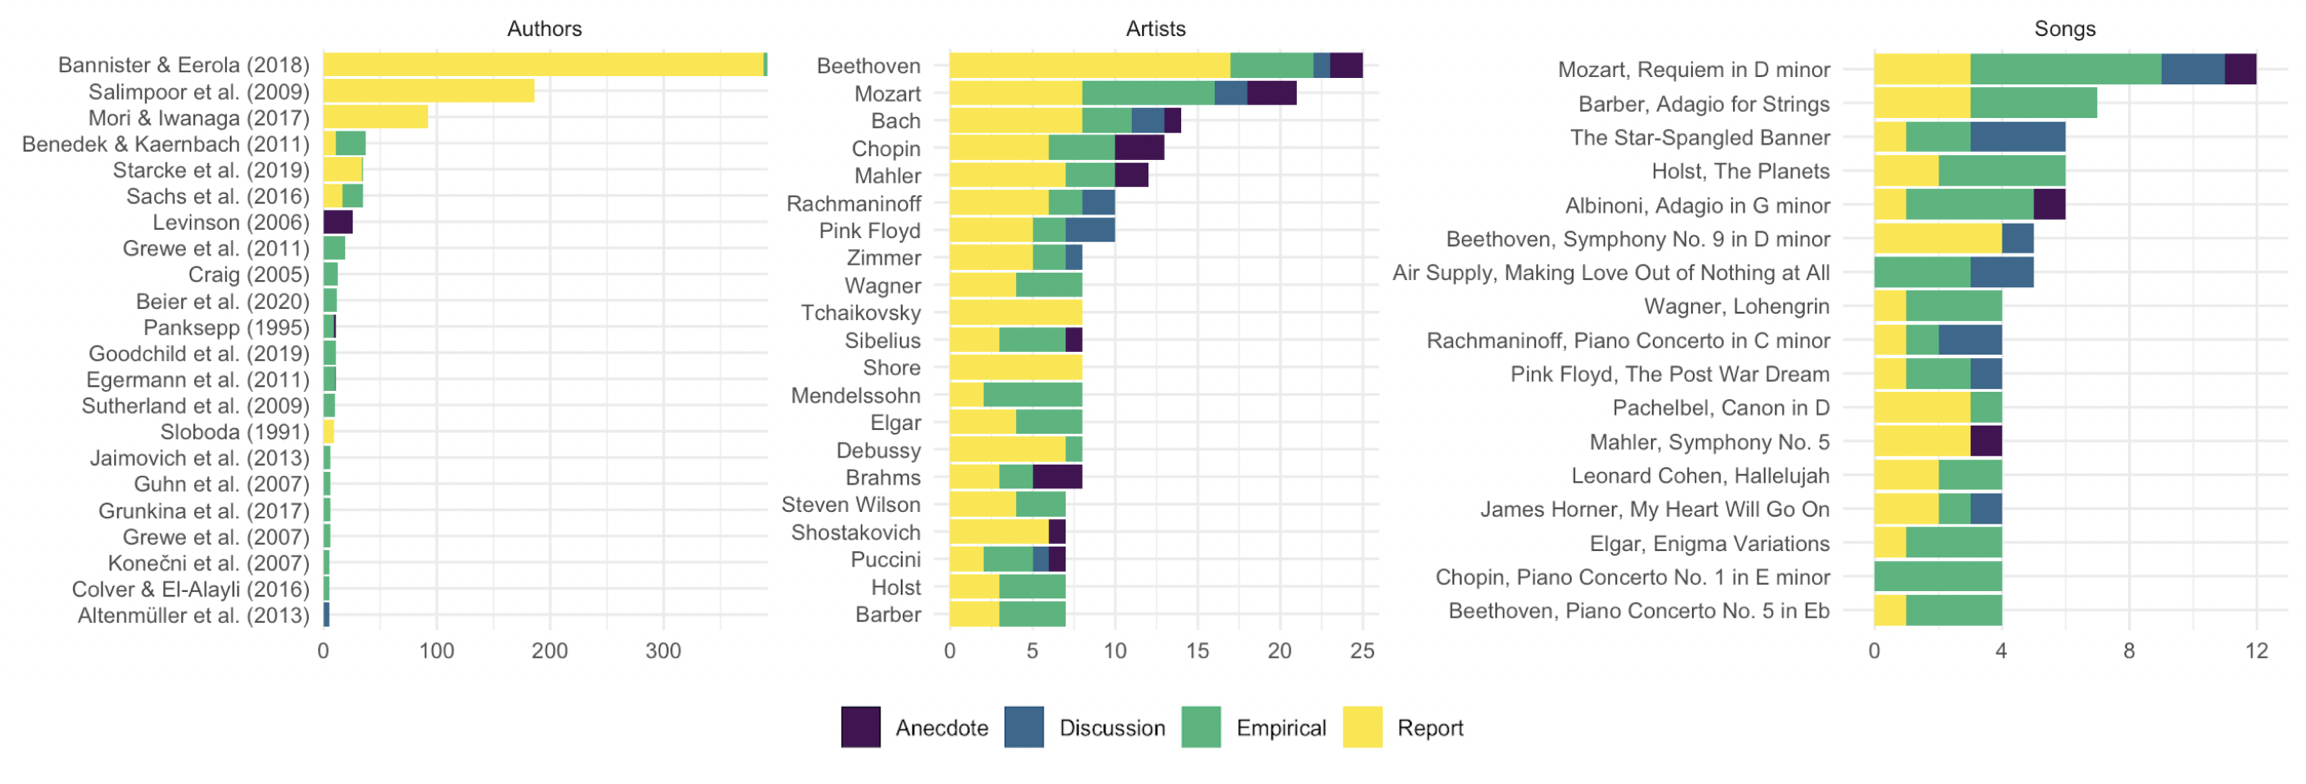
\includegraphics[width=\textwidth]{val-1.png}
\centering
\caption{Count of pieces of music in version 1.0.0 of ChiM. The first plot shows the source of most items in ChiM, with more than 500 pieces of music originating from two articles only. The two other plots show the most frequent composers and pieces of music in ChiM. The colours in each bar represent whether a piece of music was an anecdote by the authors, a participant report of MECs, an empirical verification of MECs, or a discussion of prior results.}
\label{fig:val-1}
\end{figure}

\subsubsection{Features}

Track-level audio features were collected using \emph{spotifyr} \parencite{thompson2020}, an R package which enables pulling track information from the Spotify Web API. This allowed us to obtain, for most tracks, a range of features of interest, including \emph{duration} (in milliseconds) and \emph{popularity} (based on number and recency of plays), as well as nine track-level audio features: \emph{acousticness} (confidence that the track is acoustic), \emph{danceability} (based on tempo, rhythm stability, beat strength, and overall regularity), \emph{energy} (based on dynamic range, perceived loudness, timbre, onset rate, and general entropy), \emph{instrumentalness} (confidence that the track contains no vocal content), \emph{liveness} (likelihood that the track was performed live), \emph{loudness} (overall loudness in decibels), \emph{speechiness} (presence of spoken words), \emph{valence} (conveyed musical positiveness), and \emph{tempo} (estimated in beats per minute). While Spotify does not share details about how these audio features are computed, they have been used successfully in previous research \parencite[e.g.,][]{masherrero2018, melchiorre2020}.

\subsection{Matching procedure}
\label{se:val-matching}

\subsubsection{Chills source}

We removed 136 duplicated tracks from ChiM, before looking up track information by sending API queries for strings containing the artist (or arranger/interpreter, as indicated in ChiM) and title of each track. The top result for each query was retained, and used to pull the features described above. Throughout this process, an additional 103 tracks were removed due to unavailability on Spotify or missing audio features, resulting in a dataset of 749 tracks which can cause MECs.

\subsubsection{Matched source}
\label{se:val-matching-2}

Our analysis aimed to identify if specific track-level features were related to the occurrence of MECs in ChiM. Therefore, a control set of tracks which do not cause MECs was needed. Since it is impossible to assert that a specific track never causes MECs for anyone, we approximated the construction of this control set. More specifically, we compared features across tracks from the chills source with features in another set of tracks, matched as fairly as possible with the chills source by artist, duration, and popularity. This strict matching procedure ensured there were as few differences as possible between both sets of tracks other than their potential to elicit MECs. While it is possible that some tracks from the matched source could elicit MECs as well (see Chapter \ref{ch:3} and the discussion in this chapter for some limitations in our approach), it is unlikely that all of them would, meaning that any difference detected between the two sets of tracks should shed light on which factors affect the occurrence of MECs. 

We decided to improve the matching approach used in Chapter \ref{ch:3} by implementing an algorithmic matching method. First, we gathered potential matches by getting the first 50 tracks for each of the first 50 albums returned by an API query for each artist represented in the tracks from the chills source. Then, we removed from these potential matches any track which was already present in the chills source, by comparing Spotify track IDs across the two sets. However, many duplicates remained across the two sets, since a piece of music on Spotify can have several distinct track IDs or slightly different titles. In order to mitigate this possibility, for each artist, we also removed from the potential matches any track with a title that had any number or any word of four letters or more (except the words \emph{major} and \emph{minor}) in common with tracks from the chills source. This process resulted in a pool of 205,717 potential matches.

Finally, we standardised track duration and popularity across tracks from the chills source and the potential matches. For each artist, the potential matches with the shortest Euclidean distance from each track from the chills source for these two standardised features were retained as the best matches. Audio features were pulled for these 749 matches, but were missing for 10 of them. A further 17 matches were considered as outliers and removed for having Euclidean distances larger than three standard deviations from the mean, resulting in 722 pairs of tracks from the chills and matched sources. The matching procedure is illustrated in \autoref{fig:val-2}, and the full list of tracks from the chills and matched sources is included in the supplementary materials of the published article corresponding to this chapter \parencite{defleurian2021a}.\footnote{This list of tracks is not included as an appendix to the present thesis due to its large size, better suited for a CSV-formatted file.}

\begin{figure}[t!]
\centering
\begin{subfigure}[t]{\textwidth}
    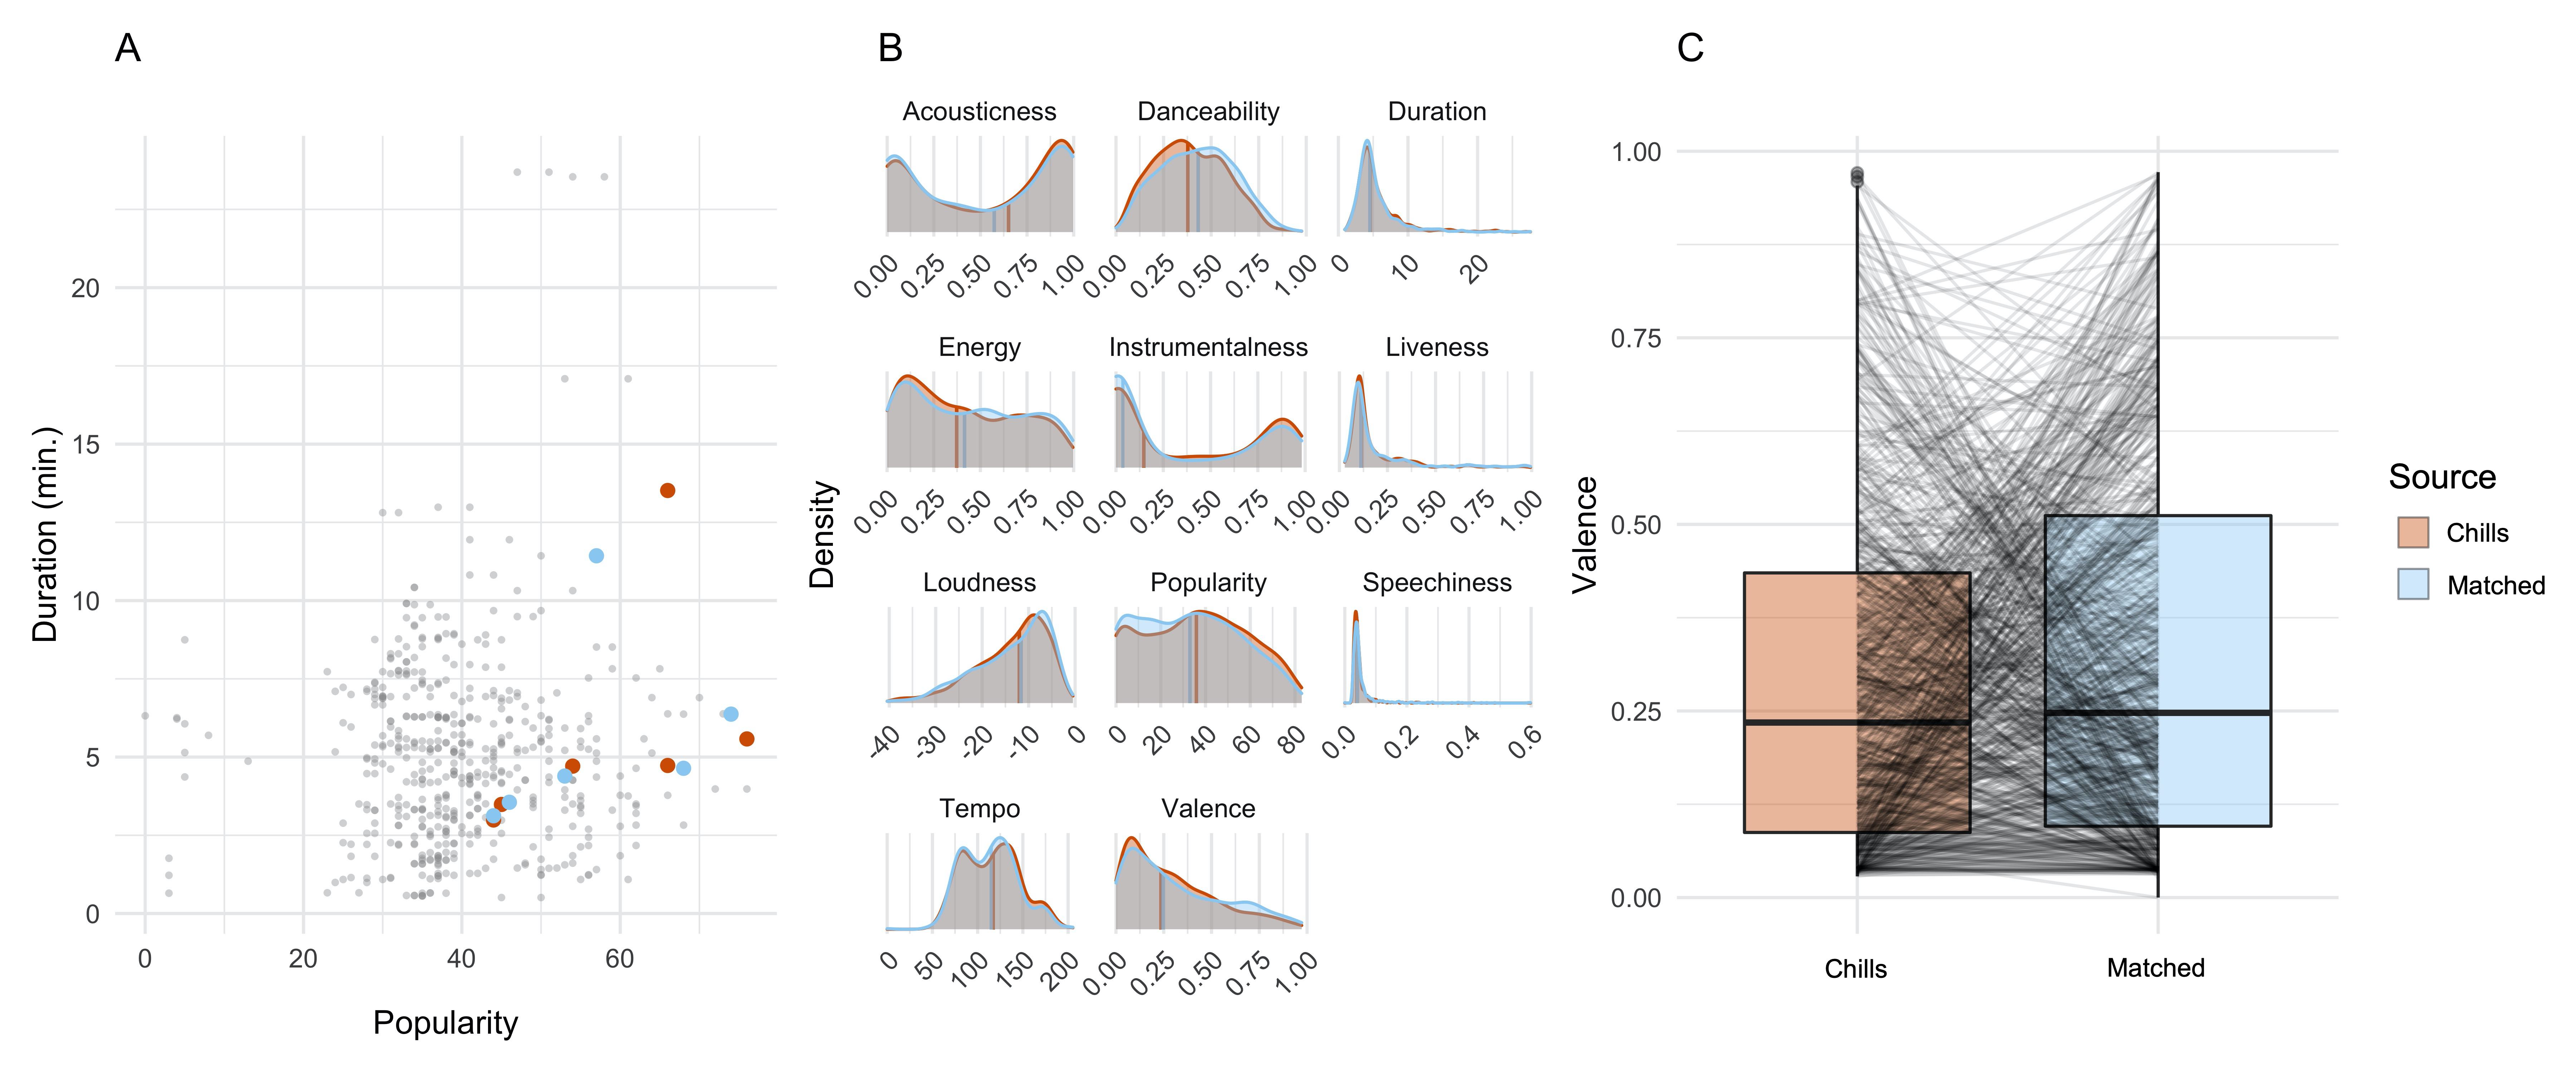
\includegraphics[width=\textwidth]{val-2.jpg}
    \phantomcaption
\end{subfigure}
\begin{subfigure}[t]{0\textwidth}
    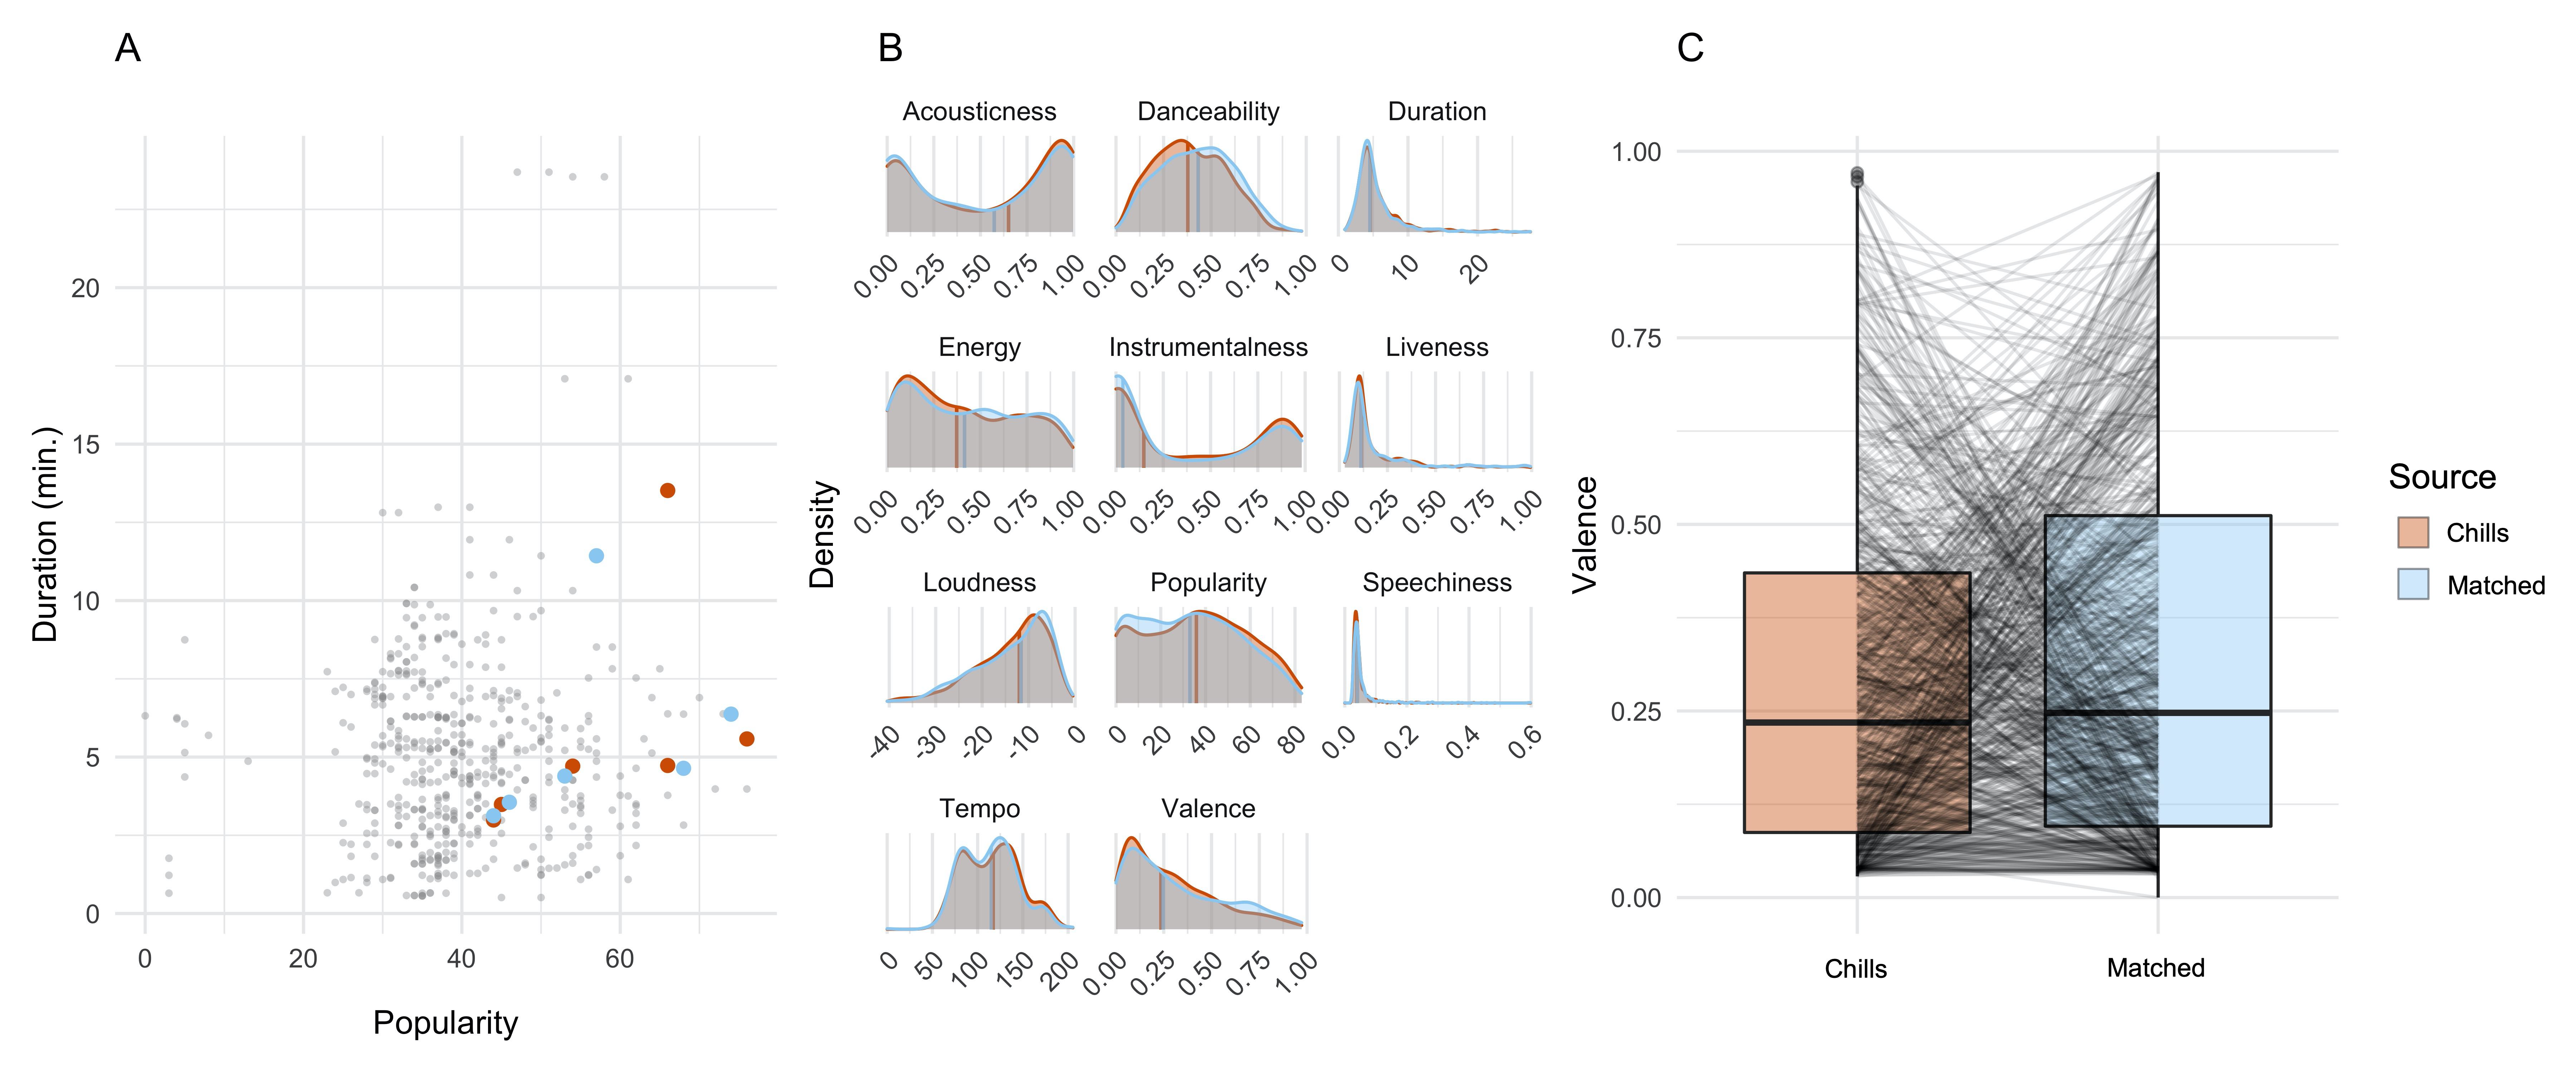
\includegraphics[width=\textwidth]{val-2.jpg}
    \phantomcaption
\end{subfigure}
\begin{subfigure}[t]{0\textwidth}
    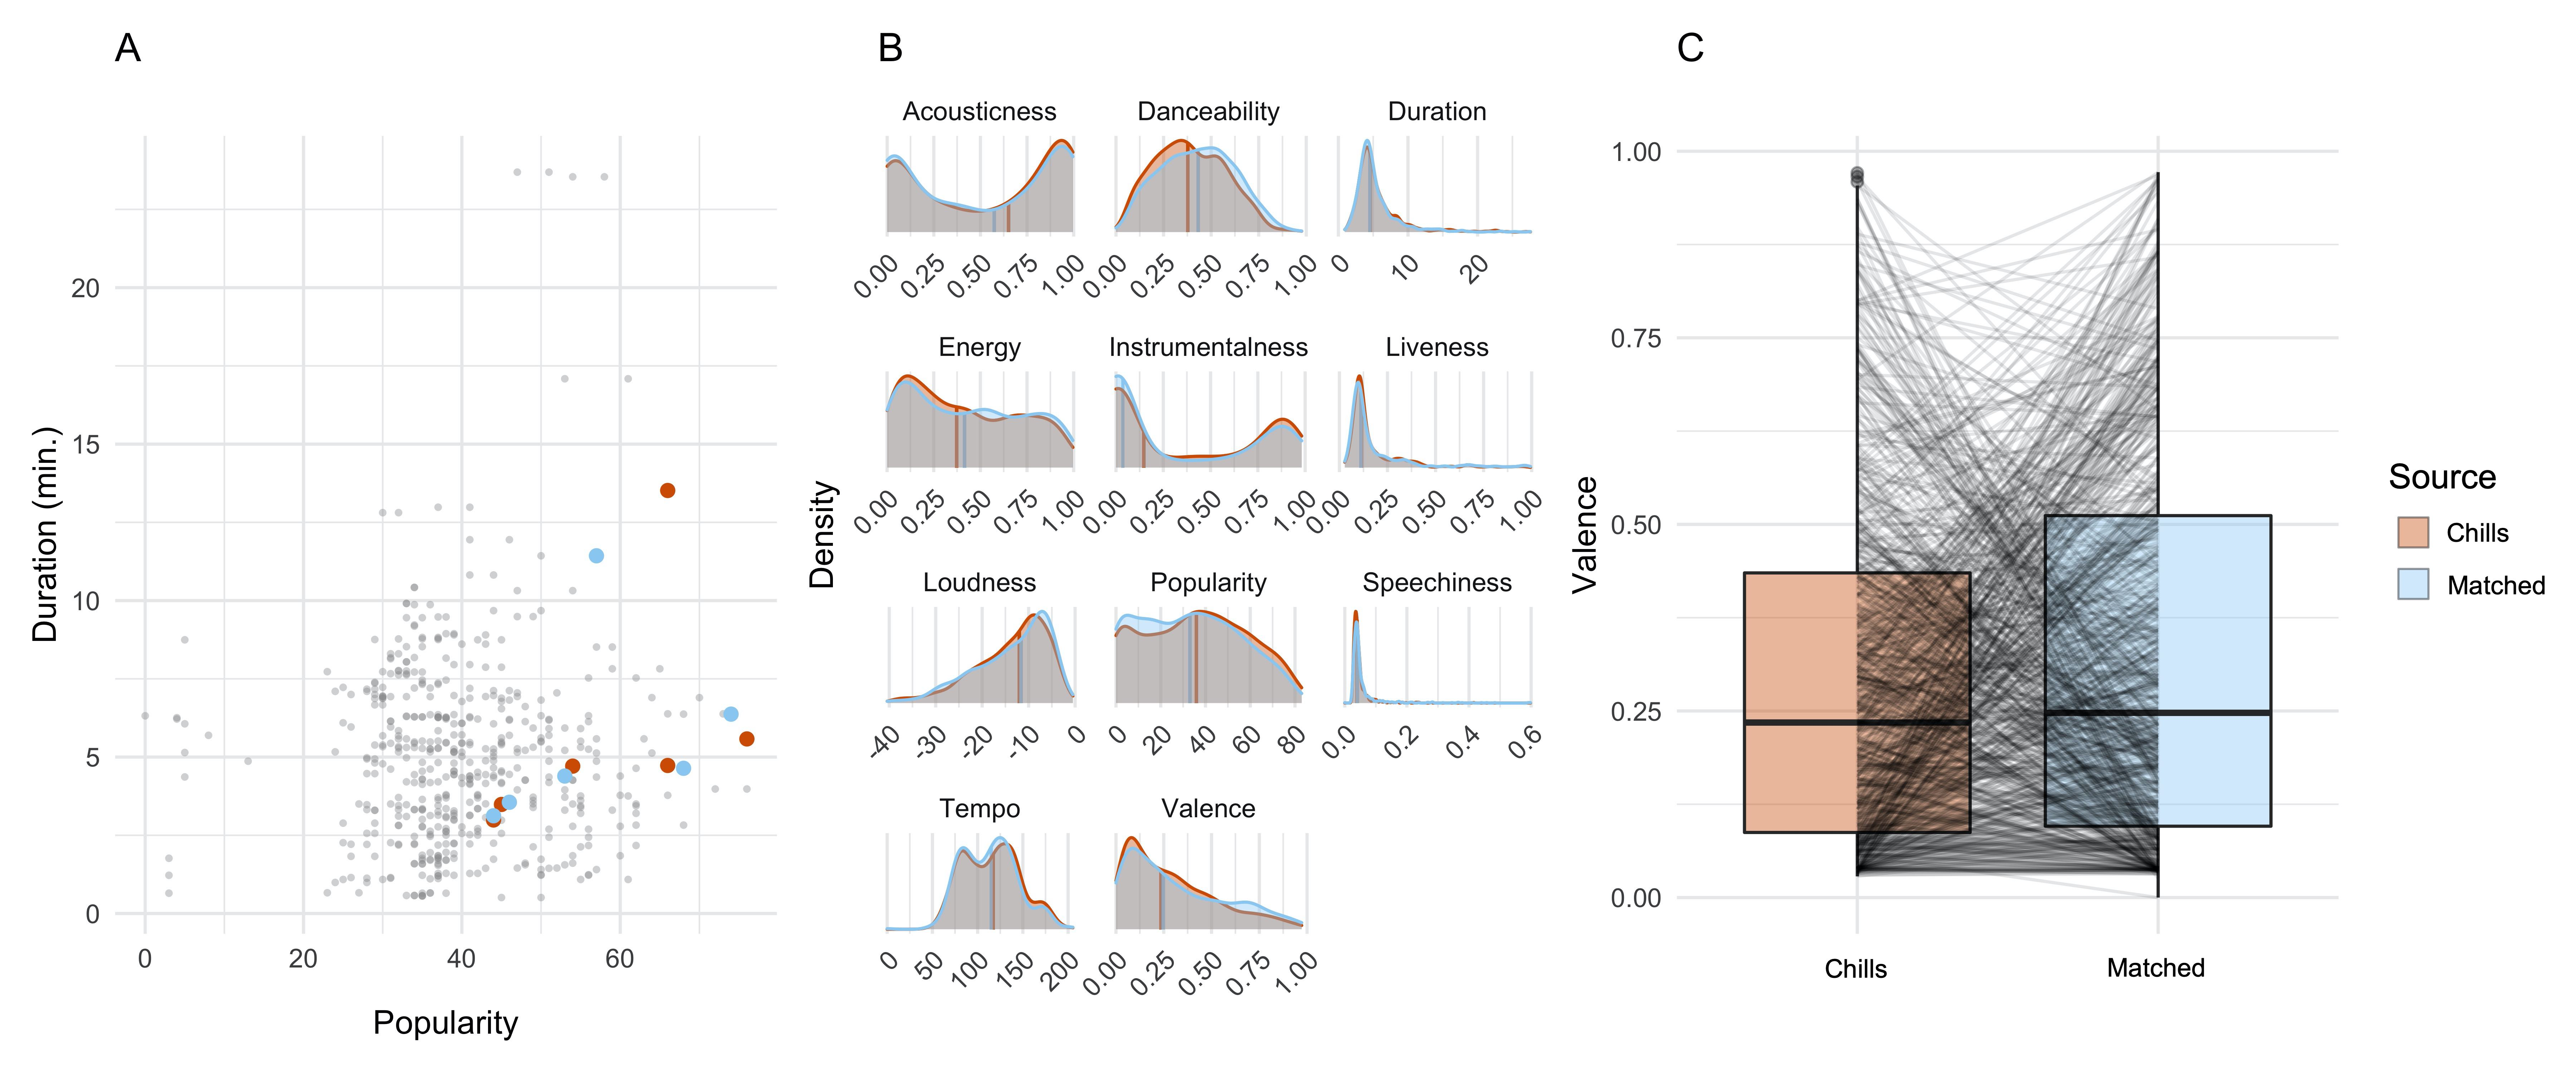
\includegraphics[width=\textwidth]{val-2.jpg}
    \phantomcaption
\end{subfigure}
\caption{\textbf{A.} Example of the matching procedure, using Pink Floyd tracks. Tracks from ChiM are shown in orange, and potential matches gathered with the Spotify Web API are shown in grey. Potential matches with the shortest Euclidean distance from each track from the chills source, in terms of duration and popularity, were selected as matches, shown in blue. \textbf{B.} Densities and median values of audio features and metadata for the 722 resulting pairs of tracks from the chills and matched sources. \textbf{C.} Boxplots showing valence for the 722 pairs of tracks, with lines linking valence scores for each individual pair.}
\label{fig:val-2}
\end{figure}

\section{Analysis}
\label{se:val-methods-3}

The confirmatory analysis consisted of assessing whether there was a difference in valence between tracks from the chills and matched sources. We ran a logistic regression for the effect of the valence feature on track source (chills vs. matched). The presence of influential data points was checked with leave-one-out diagnostics, with the plan to run another logistic regression excluding data points that would, if left out, affect the slope by at least half of its original absolute value.

The exploratory analyses were twofold. First, we assessed whether there was a difference between 
tracks from the chills and matched sources in the nine audio features described earlier. Due to high collinearity between these features (see \autoref{fig:val-3}), we first ran a principal component analysis (PCA), a method which projects each data point into a new dimensional space, the axes of which are called principal components, and allows for dimensionality reduction when retaining the first few components, which account for as much variance in the data as possible. PCA was run with centring and scaling, resulting in two principal components with eigenvalues above one---a common threshold to decide which components to retain based on how much variance they explain in the original data. We ran a logistic regression for the effects of these two principal components on track source (chills vs. matched), checking influential data points with leave-one-out diagnostics as described above.

\begin{figure}[t!]
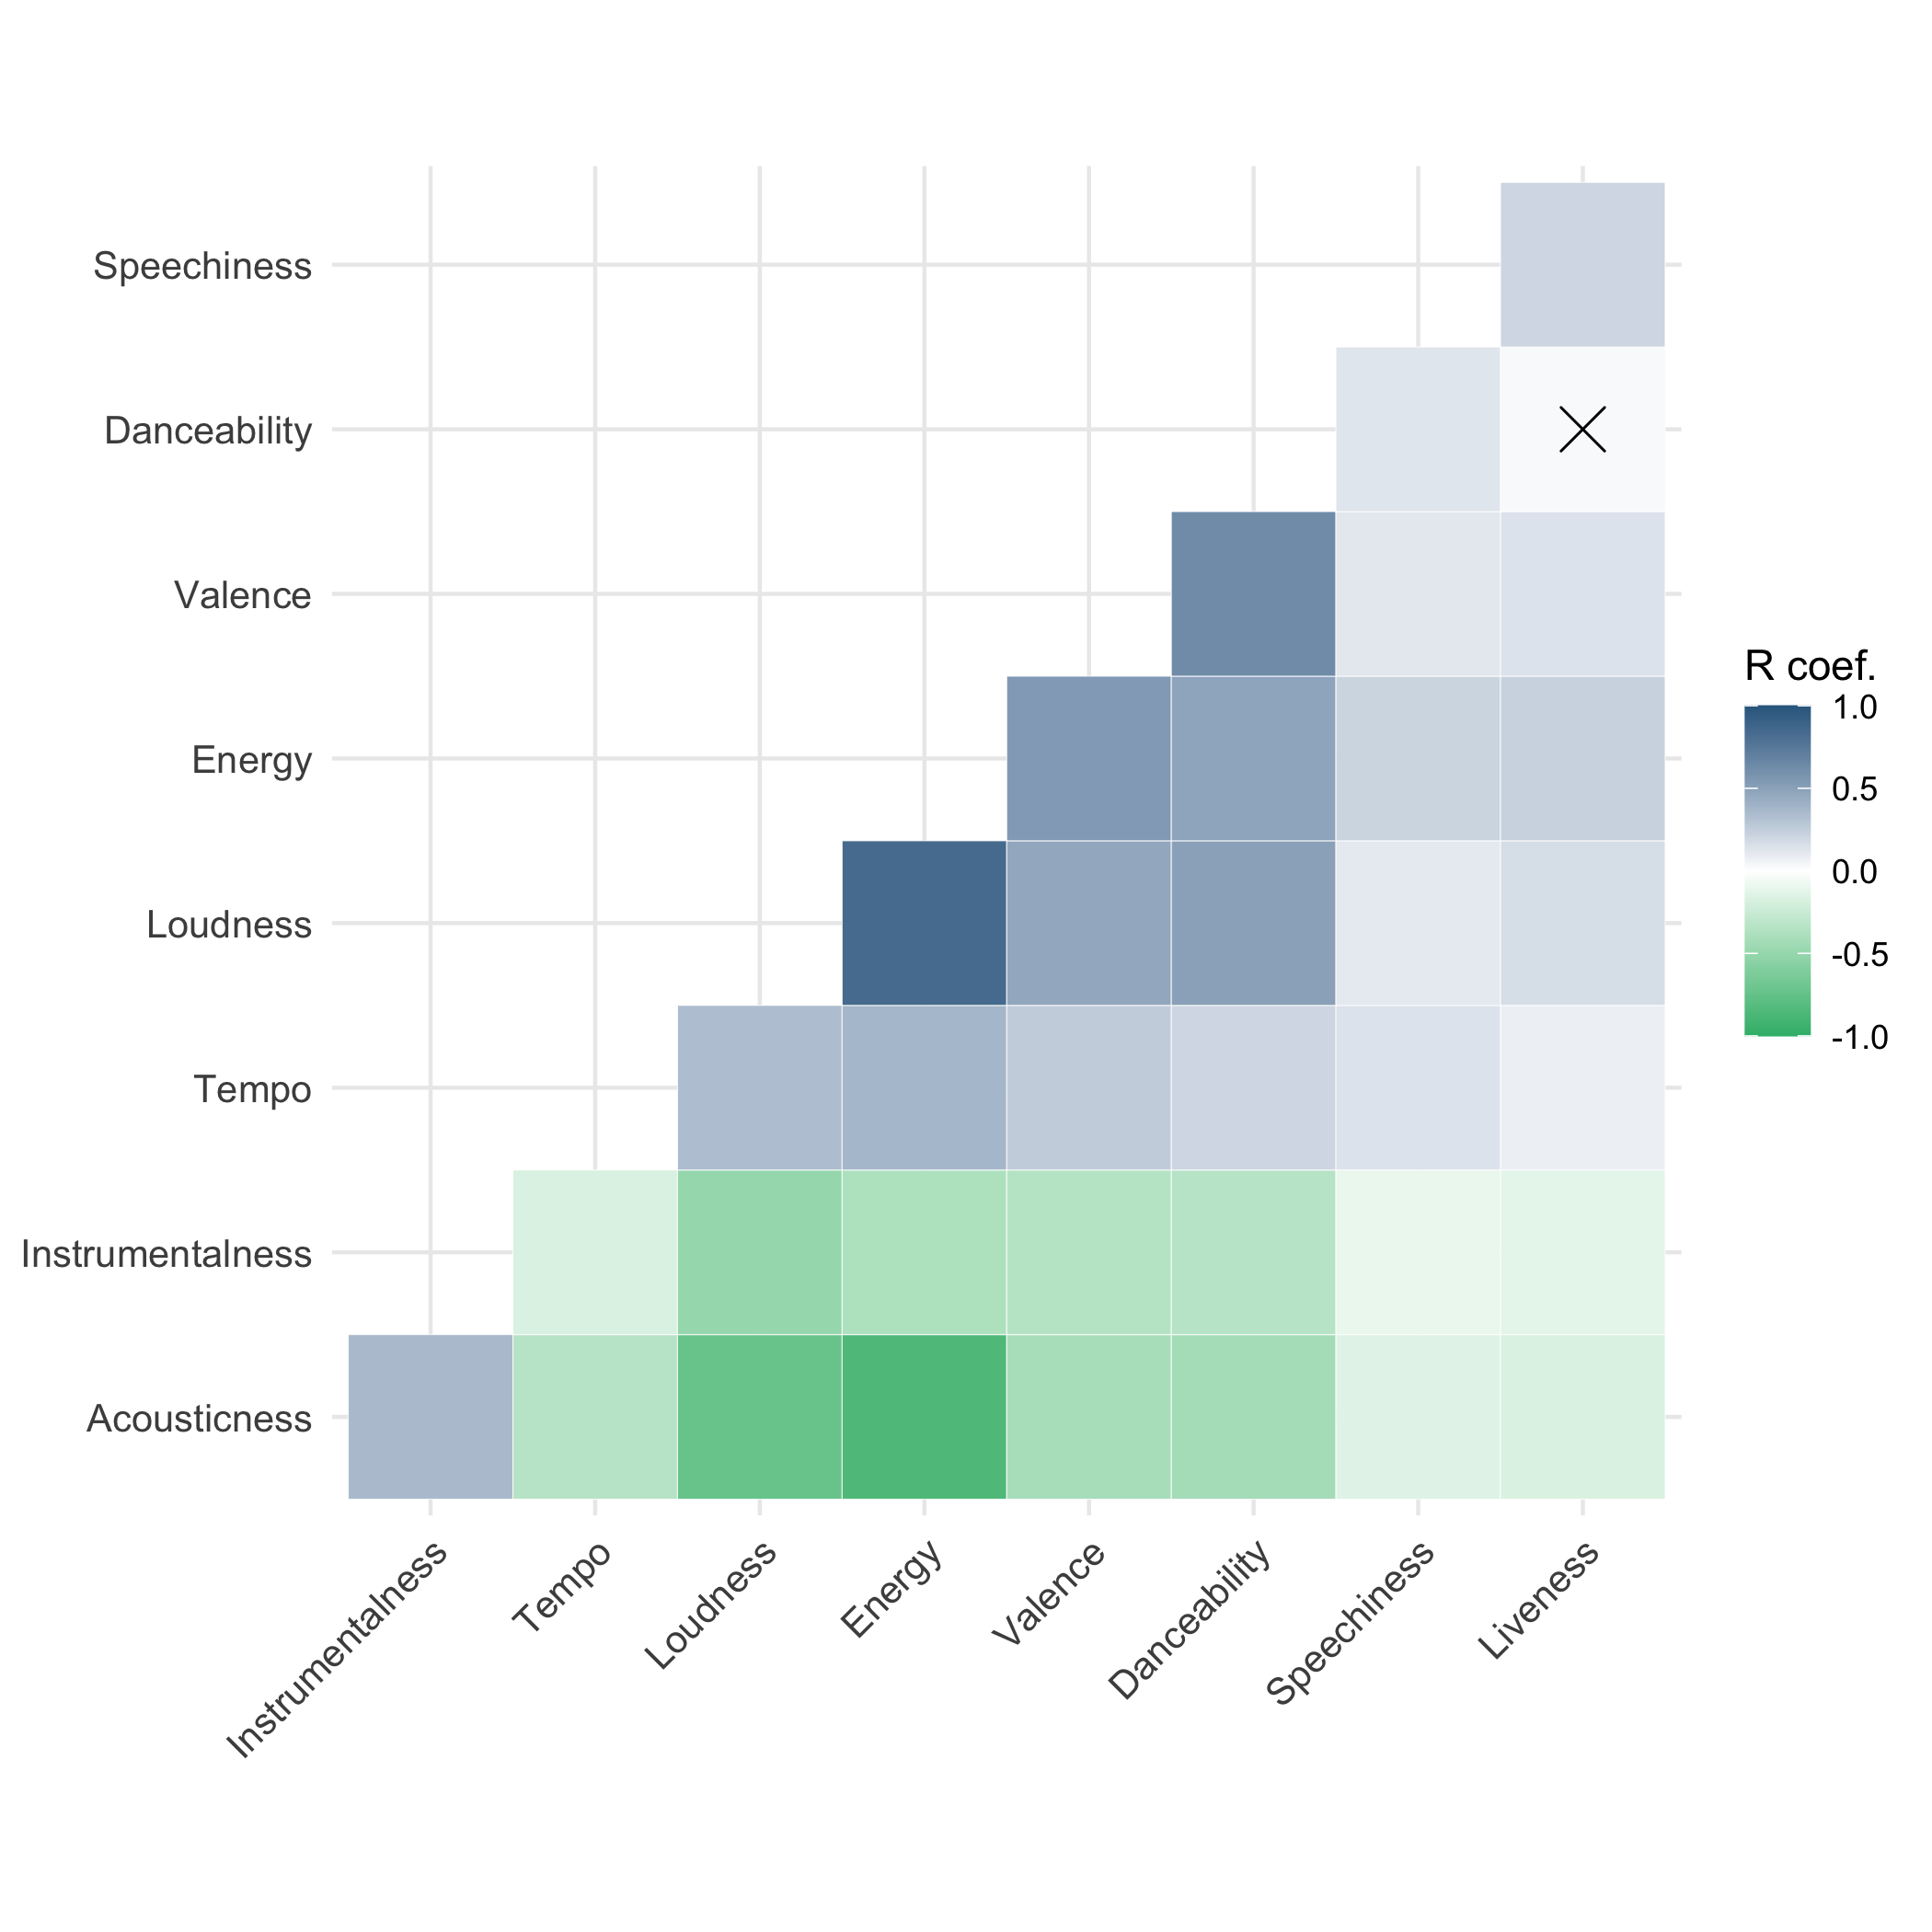
\includegraphics[width=\textwidth]{val-3.png}
\centering
\caption{Correlation matrix, showing the high degree of collinearity between each feature. Positive correlations are shown in blue and negative correlations in green. Colour saturation corresponds to the magnitude of each correlation, and the only non-significant correlation is indicated by a cross in the corresponding cell.}
\label{fig:val-3}
\end{figure}

Second, we assessed whether the audio features of the tracks from the chills source had an effect on the \emph{difference} in valence between tracks from the chills and matched sources, which could possibly mean that different types of MECs arise in response to different auditory characteristics. As described above, we first ran a PCA due to collinearity, before running a linear regression for the effects of the two resulting principal components on the difference in valence between the tracks from the chills and matched sources, using leave-one-out diagnostics, and checking homoscedasticity and normality of residuals with residuals plots.

Finally, to check the robustness of the matching procedure, we conducted Wilcoxon signed-rank tests to compare duration and popularity between tracks from the chills and matched sources, expecting no significant differences in duration and popularity. Nonparametric tests were chosen due to the fact that duration and popularity did not follow a normal distribution (see \autoref{fig:val-2}). Since there were some differences between both sets of tracks (see Section \ref{se:val-results-2}), we conducted mediation analyses, using the nonparametric bootstrap with 5000 Monte Carlo draws, as implemented in the \emph{mediation} R package \parencite{tingley2014}, to check if potential effects of the valence feature on track source were mediated by track duration and popularity. Mediation analysis enables the separation of the total effect into average causal mediation effect (ACME, the indirect effect of the independent variable on the dependent variable that goes through the mediator) and average direct effect (ADE, the direct effect of the independent variable on the dependent variable). In addition, to mitigate this weakness of the matching procedure, all the analyses described above were replicated a total of 10 times, using a different set of matched sources, each comprising one of the 10 tracks with the shortest Euclidean distance from each track from the chills source (i.e., shortest Euclidean distance for iteration \#1, second shortest for iteration \#2, etc.)

\section{Results}
\label{se:val-results}

\subsubsection{Effect of valence on track source}

A logistic regression model yielded a significant fit ($\chi^2(1) = 6.33$, $p = .012$, Nagelkerke $R^2 = .006$), revealing a significant effect of the valence feature on track source ($b = 0.54$, $Z = 2.51$, $p = .012$), with the valence of tracks from the chills source being lower than that of tracks from the matched source by 0.033 on a 0--1 scale (see \autoref{fig:val-2}). This effect remained significant across all 10 iterations of the analysis (mean valence difference $= 0.042$, $SD = 0.009$). Results for the 10 iterations are shown in \autoref{tab:val-1}.

\begin{table}[h]
\centering
\small

\begin{threeparttable}
\caption{Effect of valence on track source}
\label{tab:val-1}

\begin{tabular*}{\textwidth}{@{\extracolsep{\fill}}lrrrrrr@{}}
\toprule & 
\multicolumn{3}{l}{\textbf{Model fit}} & \multicolumn{3}{l}{\textbf{Valence}} \\ 
\cmidrule{2-7}

Iteration & $\chi^2$ & $p$      & Nagelkerke $R^2$ & $b$       & $Z$       & $p$          \\ 
\midrule

1         & 6.33     & .012     & .006             & 0.54      & 2.51      & .012         \\
2         & 12.04    & $<$ .001 & .011             & 0.75      & 3.45      & $<$ .001     \\
3         & 8.99     & .003     & .008             & 0.65      & 2.99      & .003         \\
4         & 5.13     & .023     & .005             & 0.51      & 2.26      & .024         \\
5         & 13.13    & $<$ .001 & .012             & 0.80      & 3.60      & $<$ .001     \\
6         & 6.42     & .011     & .006             & 0.56      & 2.53      & .012         \\
7         & 11.72    & $<$ .001 & .011             & 0.75      & 3.40      & $<$ .001     \\
8         & 15.46    & $<$ .001 & .014             & 0.83      & 3.91      & $<$ .001     \\
9         & 15.88    & $<$ .001 & .015             & 0.86      & 3.96      & $<$ .001     \\
10        & 14.98    & $<$ .001 & .014             & 0.84      & 3.84      & $<$ .001     \\ 
\bottomrule

\end{tabular*}
\end{threeparttable}
\end{table}

\subsubsection{Mediating effects of duration and popularity}
\label{se:val-results-2}

A Wilcoxon signed-rank test revealed no significant difference in duration ($V = 137199$, $p = .232$) and a significant difference in popularity ($V = 134593$, $p = .003$) between tracks from the chills and matched sources (higher for the chills source by 2.90 on a 1--100 scale), suggesting that the matching procedure did not result in an optimal set of matched tracks. The difference in popularity remained significant in all 10 iterations of the analysis, while the difference in duration became significant in the fourth as well as the last five iterations of the analysis, presumably due to the increasing Euclidean distance between tracks from the chills source and each successive set of matched sources (see \autoref{tab:val-2}).

\begin{table}[h]
\centering
\small

\begin{threeparttable}
\caption{Difference in duration and popularity between track sources}
\label{tab:val-2}

\begin{tabular*}{\textwidth}{@{\extracolsep{\fill}}lrrrr@{}}

\toprule & 
\multicolumn{2}{l}{\textbf{Duration}} & \multicolumn{2}{l}{\textbf{Popularity}} \\ 
\cmidrule{2-5}

Iteration & $V$                & $p$              & $V$               & $p$                 \\ 
\midrule

1         & 137199             & .232             & 134593            & .003                \\
2         & 142583             & .051             & 145166            & $<$ .001            \\
3         & 142185             & .060             & 150597            & $<$ .001            \\
4         & 146264             & .005             & 152310            & $<$ .001            \\
5         & 140323             & .059             & 154629            & $<$ .001            \\
6         & 141824             & .026             & 159205            & $<$ .001            \\
7         & 145974             & .005             & 159076            & $<$ .001            \\
8         & 144000             & .013             & 162740            & $<$ .001            \\
9         & 143062             & .010             & 163894            & $<$ .001            \\
10        & 144711             & .004             & 165209            & $<$ .001            \\ 
\bottomrule

\end{tabular*}
\end{threeparttable}
\end{table}

To assess whether duration and popularity mediated the effect of the valence feature on track source as reported above, we conducted two separate causal mediation analyses. For duration, the average causal mediation effect was not significant ($ACME = -.006$, $p = .716$) and the average direct effect was significant ($ADE = -.128$, $p = .021$), suggesting that duration did not mediate the effect of valence on track source. For popularity, both average effects were significant ($ACME = .037$, $p = .002$; $ADE = -.171$, $p < .001$), suggesting that popularity partially, but not fully, mediated the effect of valence on track source. These results remained stable across the 10 iterations of the analysis, except for duration, which partially mediated the effect of valence on track source in the last iteration (see \autoref{tab:val-3}).

\begin{table}[ht]
\centering
\small

\begin{threeparttable}
\caption{Mediation analyses for the effect of valence on track source}
\label{tab:val-3}

\begin{tabular*}{\textwidth}{@{\extracolsep{\fill}}lrrrrrrrr@{}}

\toprule & 
\multicolumn{4}{l}{\textbf{Duration}} & \multicolumn{4}{l}{\textbf{Popularity}} \\ 
\cmidrule{2-9}

Iteration & $ACME$   & $p$   & $ADE$  & $p$       & $ACME$  & $p$       & $ADE$  & $p$      \\ 
\midrule

1         & -.006    & .716  & -.128  & .021      & .037    & .002      & -.171  & $<$ .001 \\
2         & -.010    & .503  & -.173  & .002      & .049    & $<$ .001  & -.232  & $<$ .001 \\
3         & -.012    & .434  & -.147  & .004      & .063    & $<$ .001  & -.223  & .001     \\
4         & -.028    & .103  & -.100  & .095      & .067    & $<$ .001  & -.196  & $<$ .001 \\
5         & -.012    & .419  & -.184  & $<$ .001  & .073    & $<$ .001  & -.270  & $<$ .001 \\
6         & -.020    & .232  & -.118  & .034      & .072    & $<$ .001  & -.209  & $<$ .001 \\
7         & -.019    & .209  & -.164  & .002      & .073    & $<$ .001  & -.256  & $<$ .001 \\
8         & -.016    & .267  & -.189  & $<$ .001  & .075    & $<$ .001  & -.281  & $<$ .001 \\
9         & -.022    & .145  & -.188  & .001      & .073    & $<$ .001  & -.285  & $<$ .001 \\
10        & -.032    & .046  & -.174  & .002      & .081    & $<$ .001  & -.288  & $<$ .001 \\ 
\bottomrule

\end{tabular*}
\end{threeparttable}
\end{table}

In this case, the mediation analyses each involved a linear regression (for the effect of valence on duration/popularity) and a logistic regression (for the effects of valence and duration/popularity on track source). It is worth noting that for the linear models, some assumptions (homoscedasticity and normality of residuals) were violated, as shown in \autoref{fig:val-4}. This was most likely due to the distribution of valence, duration, and popularity in our data (see \autoref{fig:val-2}). To confirm the results of the mediation analyses, we ran them again on a reduced (keeping only tracks with non-zero popularity due to this feature being zero-inflated) and transformed dataset (square root for popularity and log for valence and duration). These re-analyses did not fully eliminate the violations of assumptions for linear regression, but did replicate the findings presented above (see \autoref{tab:val-4}).

\begin{figure}[t!]
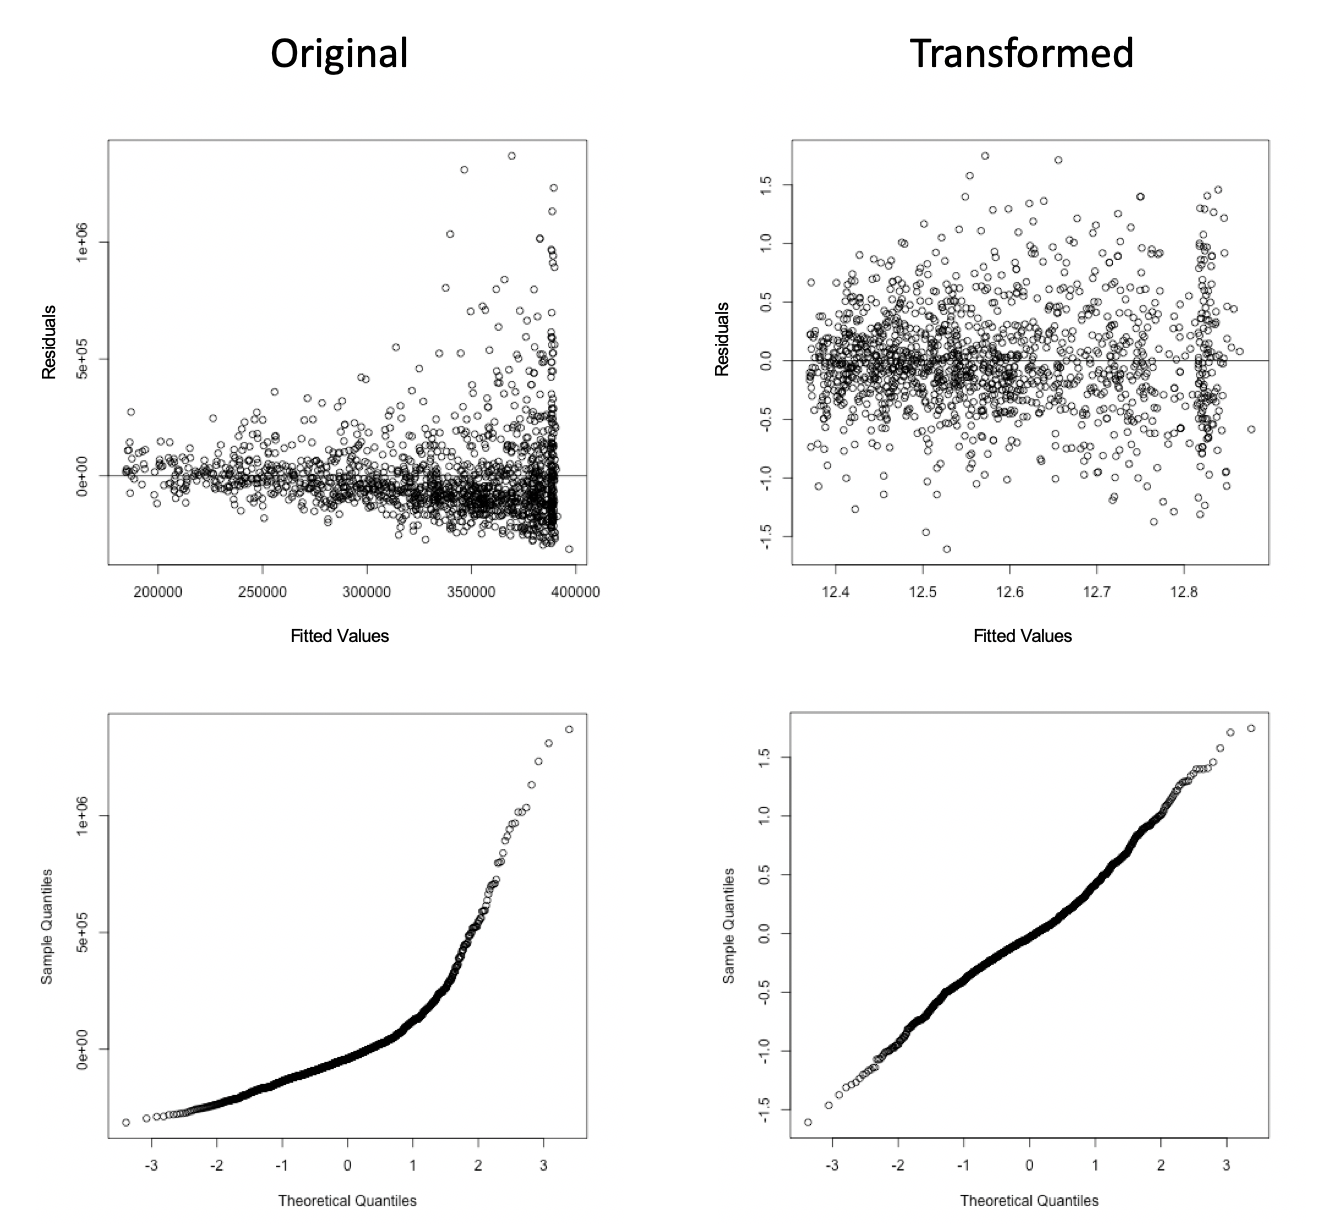
\includegraphics[width=\textwidth]{val-4.png}
\centering
\caption{Diagnostic plots for a linear regression of the effect of valence on track duration. Plots on the left show a violation of homoscedasticity in the top residuals plot, and a violation of normality in the bottom Normal Q-Q plot when using untransformed variables. Plots on the right show that, when using log-transformed variables for valence and track duration instead, the assumptions for linear regression were much better fulfilled. Note that these improvements were not as noticeable for all models.}
\label{fig:val-4}
\end{figure}

\begin{table}[h]
\centering
\small

\begin{threeparttable}
\caption{Mediation re-analyses for the effect of valence on track source}
\label{tab:val-4}

\begin{tabular*}{\textwidth}{@{\extracolsep{\fill}}lrrrrrrrr@{}}

\toprule & 
\multicolumn{4}{l}{\textbf{Duration}} & \multicolumn{4}{l}{\textbf{Popularity}} \\
\cmidrule{2-9}

Iteration & $ACME$    & $p$    & $ADE$   & $p$    & $ACME$  & $p$       & $ADE$  & $p$      \\ 
\midrule

1         & -.002     & .656   & -.023   & .109   & .010    & .001      & -.036  & .010     \\
2         & -.005     & .304   & -.034   & .024   & .013    & $<$ .001  & -.052  & $<$ .001 \\
3         & -.006     & .136   & -.019   & .174   & .017    & $<$ .001  & -.043  & .002     \\
4         & -.009     & .086   & -.024   & .102   & .020    & $<$ .001  & -.052  & $<$ .001 \\
5         & -.006     & .217   & -.030   & .032   & .020    & $<$ .001  & -.056  & $<$ .001 \\
6         & -.007     & .094   & -.017   & .242   & .021    & $<$ .001  & -.045  & $<$ .001 \\
7         & -.008     & .051   & -.028   & .058   & .023    & $<$ .001  & -.059  & $<$ .001 \\
8         & -.005     & .198   & -.028   & .049   & .023    & $<$ .001  & -.056  & $<$ .001 \\
9         & -.008     & .070   & -.036   & .014   & .021    & $<$ .001  & -.065  & $<$ .001 \\
10        & -.010     & .026   & -.036   & .016   & .026    & $<$ .001  & -.072  & $<$ .001 \\ 
\bottomrule

\end{tabular*}
\end{threeparttable}
\end{table}

\subsubsection{Effects of audio features on track source}
\label{se:val-results-3}

We ran a PCA to reduce collinearity in the nine audio features. We retained two principal components with eigenvalues higher than one, accounting for 56.4\% of cumulative proportion of variance explained \parencite[see supplementary materials discussed earlier in][for the values for each set of tracks]{defleurian2021a}. The first component featured high positive loadings (greater than .2) for energy, loudness, valence, danceability, and tempo, and high negative loadings (lower than -.2) for acousticness and instrumentalness. The second component featured high positive loadings for liveness and speechiness, and a high negative loading for danceability. The number of retained principal components and their associated loadings were consistent across all 10 iterations of the analysis (besides occasional but systematic sign differences, which are expected when conducting several PCAs---see \autoref{tab:val-5}).

\begin{table}[ht]
\centering
\scriptsize

\begin{threeparttable}
\caption{PCA on audio features for all tracks}
\label{tab:val-5}

\begin{tabular*}{\textwidth}{@{\extracolsep{\fill}}llrrrrrrrrr@{}}

\toprule && 
\multicolumn{9}{l}{\textbf{Audio feature loadings}} \\
\cmidrule{3-11}

PC & I. & Temp. & Loud. & Val. & Danc. & Ener. & Acou. & Inst. & Spee. & Live. \\ 
\midrule

1  & 1         & .242  & .439     & .353    & .346   & .457   & -.419   & -.291   & .132    & .134     \\
   & 2         & .222  & .444     & .356    & .346   & .459   & -.422   & -.298   & .128    & .118     \\
   & 3         & .233  & .438     & .350    & .343   & .458   & -.421   & -.289   & .151    & .142     \\
   & 4         & .220  & .447     & .351    & .341   & .461   & -.428   & -.300   & .112    & .117     \\
   & 5         & .221  & .442     & .356    & .343   & .461   & -.422   & -.297   & .139    & .117     \\
   & 6         & .243  & .439     & .354    & .338   & .456   & -.420   & -.292   & .153    & .124     \\
   & 7         & .231  & .439     & .346    & .341   & .459   & -.425   & -.301   & .151    & .115     \\
   & 8         & .241  & .437     & .352    & .348   & .453   & -.419   & -.302   & .135    & .125     \\
   & 9         & .220  & .441     & .356    & .348   & .456   & -.421   & -.293   & .151    & .124     \\
   & 10        & .241  & .438     & .351    & .351   & .456   & -.422   & -.292   & .130    & .122     \\
2  & 1         & .119  & -.083    & -.178   & -.275  & .048   & -.001   & .105    & .645    & .665     \\
   & 2         & .158  & .078     & .080    & .148   & .003   & -.071   & .046    & -.660   & -.706    \\
   & 3         & .138  & -.029    & -.293   & -.365  & .081   & -.051   & .098    & .548    & .665     \\
   & 4         & .075  & -.052    & -.240   & -.300  & .062   & -.055   & .020    & .581    & .706     \\
   & 5         & .050  & .019     & .219    & .324   & -.063  & .029    & .013    & -.567   & -.719    \\
   & 6         & .007  & -.020    & -.261   & -.359  & .076   & -.048   & .007    & .498    & .739     \\
   & 7         & .043  & -.010    & -.276   & -.363  & .048   & -.038   & -.045   & .543    & .699     \\
   & 8         & .037  & .078     & .150    & .202   & .017   & -.046   & .056    & -.644   & -.714    \\
   & 9         & .052  & -.075    & -.173   & -.267  & .020   & .012    & .035    & .612    & .717     \\
   & 10        & .088  & .100     & .101    & .162   & .007   & -.051   & .033    & -.654   & -.717 \\
\bottomrule

\end{tabular*}
\begin{tablenotes}
\small
\item Note. PC = Principal component, I. = Iteration, Temp. = Tempo, Loud. = Loudness, Val. = Valence, Danc. = Danceability, Ener. = Energy, Acou. = Acousticness, Inst. = Instrumentalness, Spee. = Speechiness, Live. = Liveness.
\end{tablenotes}
\end{threeparttable}
\end{table}

A logistic regression model yielded a significant fit ($\chi^2(2) = 6.47$, $p = .039$, Nagelkerke $R^2 = .006$), revealing a significant effect of the first component on track source ($b = 0.06$, $Z = 2.34$, $p = .019$) and no significant effect of the second component ($b = 0.05$, $Z = 0.98$, $p = .328$), showing that tracks from the chills source had lower scores than tracks from the matched source on the first component (i.e., tracks from the chills source featured lower energy, loudness, valence, danceability, and tempo, as well as higher acousticness and instrumentalness---see \autoref{fig:val-5}). The model fit remained significant in all but one iteration of the analysis ($\chi^2(2) = 5.33$, $p = .070$, Nagelkerke $R^2 = .005$), the effect of the first component remained significant in all iterations, and the effect of the second component became significant in four iterations, highlighting that in some cases, tracks from the chills source had lower scores than tracks from the matched source on the second component (i.e., low liveness and speechiness, as well as high danceability). It is worth noting that in the seventh iteration of the analysis, there were two influential data points (as described in Section \ref{se:val-methods-3}). For this iteration, we ran the model both with and without the influential data points, leading to similar results in both cases (see \autoref{tab:val-6}).

\begin{table}[ht]
\centering
\small

\begin{threeparttable}
\caption{Effects of first two principal components on track source}
\label{tab:val-6}

\begin{tabular*}{\textwidth}{@{\extracolsep{\fill}}lrrrrrrrrr@{}}

\toprule & 
\multicolumn{3}{l}{\textbf{Model fit}} & \multicolumn{3}{l}{\textbf{Component 1}} & \multicolumn{3}{l}{\textbf{Component 2}} \\
\cmidrule{2-10}

Iteration & $\chi^2$   & $p$   & Nagelkerke $R^2$  & $b$          & $Z$         & $p$         & $b$          & $Z$         & $p$         \\ 
\midrule

1  & 6.47  & .039 & .006 & 0.06 & 2.34 & .019 & 0.05  & 0.98  & .328 \\
2  & 10.39 & .006 & .010 & 0.07 & 2.42 & .016 & -0.11 & -2.10 & .036 \\
3  & 6.57  & .038 & .006 & 0.07 & 2.51 & .012 & 0.03  & 0.51  & .612 \\
4  & 13.04 & .001 & .012 & 0.07 & 2.63 & .008 & 0.12  & 2.44  & .015 \\
5  & 9.00  & .011 & .008 & 0.07 & 2.76 & .006 & -0.06 & -1.17 & .243 \\
6  & 5.33  & .070 & .005 & 0.06 & 2.15 & .032 & 0.04  & 0.83  & .404 \\
7a & 6.71  & .035 & .006 & 0.07 & 2.56 & .010 & 0.02  & 0.37  & .714 \\
7b & 6.96  & .031 & .006 & 0.07 & 2.61 & .009 & 0.02  & 0.40  & .687 \\
8  & 13.28 & .001 & .012 & 0.07 & 2.74 & .006 & -0.12 & -2.37 & .018 \\
9  & 7.20  & .027 & .008 & 0.07 & 2.61 & .009 & 0.03  & 0.60  & .551 \\
10 & 12.53 & .002 & .012 & 0.07 & 2.69 & .007 & -0.12 & -2.26 & .024 \\
\bottomrule

\end{tabular*}
\begin{tablenotes}
\small
\item Note. The analysis for iteration 7 was conducted with (7a) and without (7b) influential data points.
\end{tablenotes}
\end{threeparttable}
\end{table}

\begin{figure}[t!]
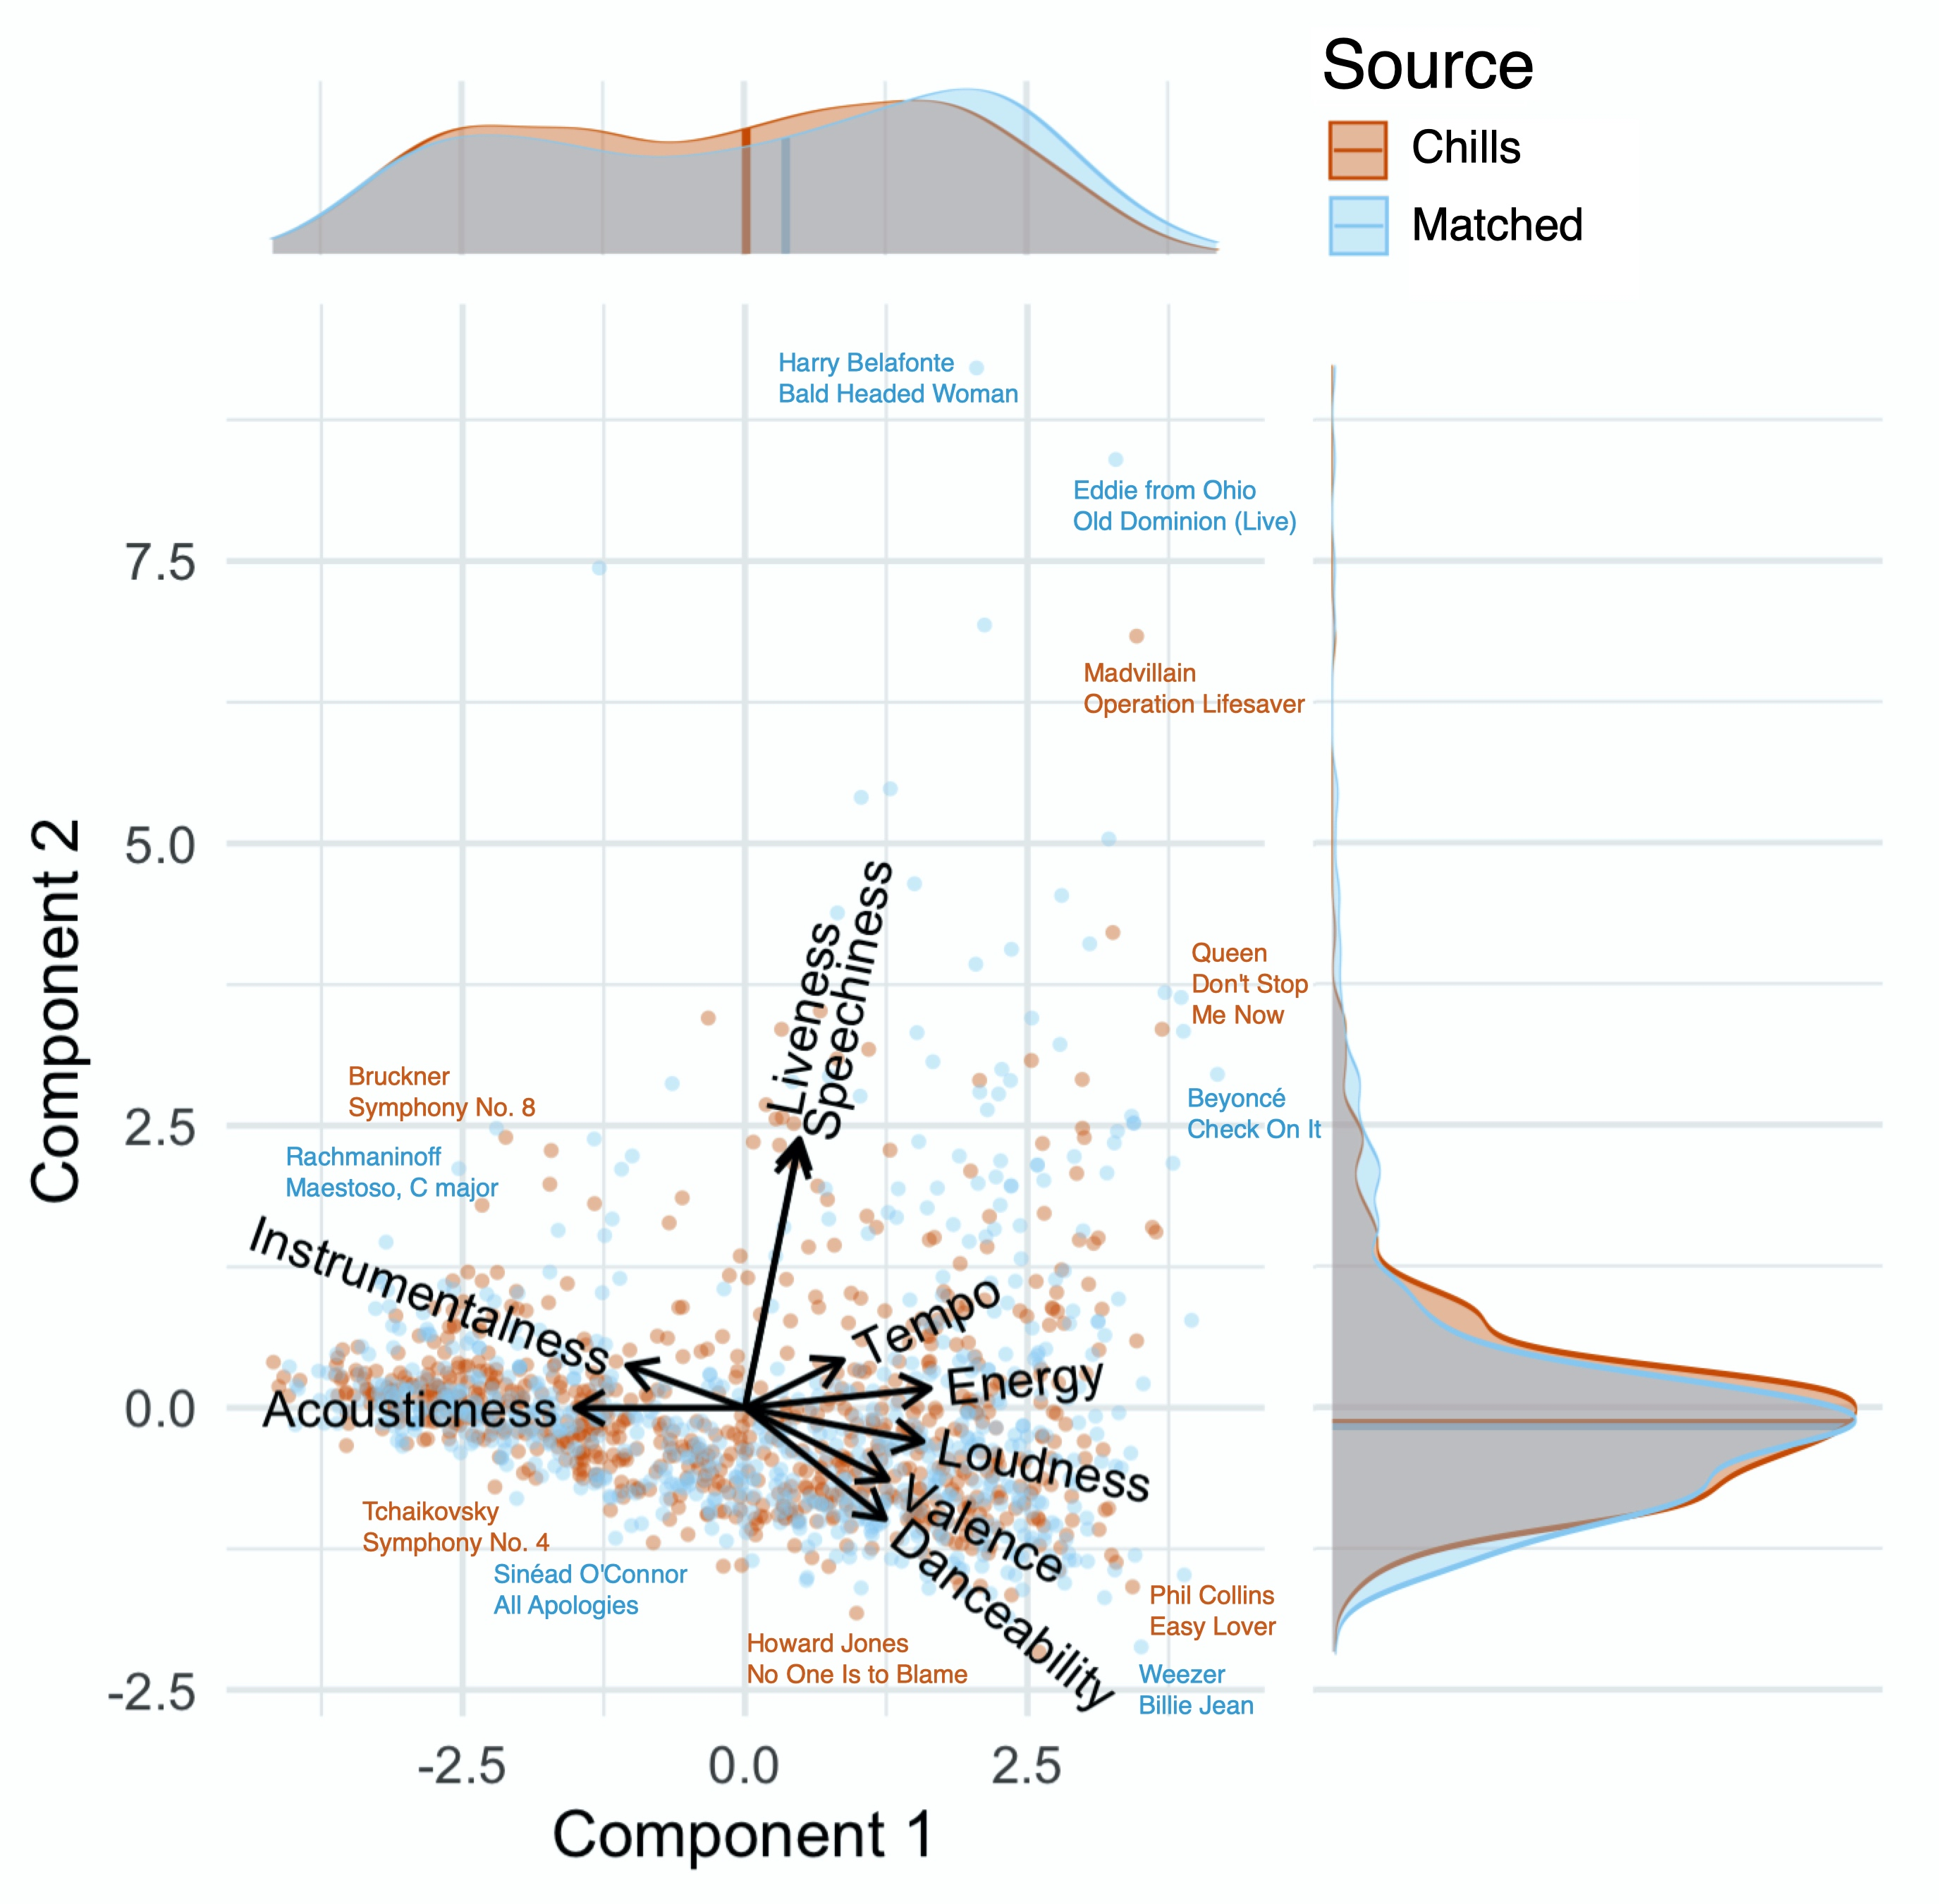
\includegraphics[width=\textwidth]{val-5.jpg}
\centering
\caption{Biplot of tracks from the chills and matched sources for the first iteration of the analysis. Tracks are mapped onto the first two components obtained with PCA. Some example tracks are shown for various combinations of component values. Densities and median values for tracks from the chills and matched sources are shown in marginal plots, revealing a difference on Component 1. Audio feature loadings are shown as vectors, illustrating the high degree of collinearity between some features.}
\label{fig:val-5}
\end{figure}

\subsubsection{Effects of audio features on difference between sources}

We ran a PCA on the nine audio features of the tracks from the chills source only (as opposed to both track sources in Section \ref{se:val-results-3}), to assess if properties of the tracks from the chills source could predict the direction and magnitude of the difference in the valence feature between both track sources. We retained two principal components with eigenvalues higher than one, accounting for 55.6\% of cumulative proportion of variance explained. Both components featured similar loadings as in the previous section. The number of retained principal components and their associated loadings were consistent across all 10 iterations of the analysis (see \autoref{tab:val-7}).

\begin{table}[ht]
\centering
\scriptsize

\begin{threeparttable}
\caption{PCA on audio features for tracks from the chills source only}
\label{tab:val-7}

\begin{tabular*}{\textwidth}{@{\extracolsep{\fill}}llrrrrrrrrr@{}}

\toprule && 
\multicolumn{9}{l}{\textbf{Audio feature loadings}} \\
\cmidrule{3-11}

PC & I. & Temp. & Loud. & Val. & Danc. & Ener. & Acou. & Inst. & Spee. & Live. \\ 
\midrule

1  & 1         & .251  & .440     & .345    & .339   & .463   & -.419   & -.283   & .155    & .126     \\
   & 2         & .249  & .440     & .346    & .336   & .463   & -.420   & -.283   & .158    & .127     \\
   & 3         & .249  & .440     & .347    & .335   & .463   & -.421   & -.283   & .157    & .125     \\
   & 4         & .247  & .441     & .346    & .334   & .464   & -.421   & -.282   & .153    & .129     \\
   & 5         & .249  & .440     & .346    & .337   & .463   & -.420   & -.281   & .156    & .129     \\
   & 6         & .253  & .439     & .344    & .337   & .463   & -.420   & -.282   & .157    & .125     \\
   & 7         & .250  & .440     & .346    & .335   & .463   & -.421   & -.282   & .158    & .126     \\
   & 8         & .250  & .440     & .346    & .335   & .463   & -.421   & -.282   & .158    & .126     \\
   & 9         & .249  & .439     & .346    & .334   & .463   & -.421   & -.285   & .159    & .126     \\
   & 10        & .250  & .438     & .345    & .338   & .462   & -.420   & -.286   & .155    & .127     \\
2  & 1         & .014  & .088     & .149    & .265   & -.020  & -.007   & -.037   & -.650   & -.690    \\
   & 2         & .008  & .083     & .164    & .283   & -.030  & .004    & -.049   & -.646   & -.682    \\
   & 3         & .009  & .081     & .164    & .281   & -.029  & .004    & -.047   & -.646   & -.684    \\
   & 4         & .005  & .084     & .162    & .284   & -.030  & .005    & -.049   & -.654   & -.674    \\
   & 5         & .025  & .086     & .148    & .273   & -.024  & -.005   & -.040   & -.648   & -.688    \\
   & 6         & .016  & .086     & .157    & .269   & -.024  & -.004   & -.040   & -.647   & -.689    \\
   & 7         & .015  & .088     & .152    & .274   & -.025  & -.001   & -.047   & -.646   & -.688    \\
   & 8         & .015  & .088     & .152    & .274   & -.025  & -.001   & -.047   & -.646   & -.688    \\
   & 9         & .009  & .084     & .162    & .277   & -.028  & .000    & -.052   & -.646   & -.685    \\
   & 10        & .011  & .082     & .160    & .277   & -.031  & .000    & -.048   & -.650   & -.682    \\
\bottomrule

\end{tabular*}
\begin{tablenotes}
\small
\item Note. PC = Principal component, I. = Iteration, Temp. = Tempo, Loud. = Loudness, Val. = Valence, Danc. = Danceability, Ener. = Energy, Acou. = Acousticness, Inst. = Instrumentalness, Spee. = Speechiness, Live. = Liveness.
\end{tablenotes}
\end{threeparttable}
\end{table}

A multiple linear regression model yielded a significant fit ($F(2, 719) = 63.9$, $p < .001$, adjusted $R^2 = .149$), revealing a significant effect for both the first component ($\beta = .062$, $p < .001$) and the second component ($\beta = .039$, $p < .001$), suggesting that tracks from the chills source with higher scores on these components were more likely to be happier than their associated tracks from the matched source, and vice versa. These effects held for all 10 iterations of the analysis (see \autoref{tab:val-8}).

\begin{table}[ht]
\centering
\small

\begin{threeparttable}
\caption{Effects of components on difference in valence between sources}
\label{tab:val-8}

\begin{tabular*}{\textwidth}{@{\extracolsep{\fill}}lrrrrrrr@{}}

\toprule & 
\multicolumn{3}{l}{\textbf{Model fit}} & \multicolumn{2}{l}{\textbf{Component 1}} & \multicolumn{2}{l}{\textbf{Component 2}} \\
\cmidrule{2-8}

Iteration & $F$  & $p$      & Adjusted $R^2$ & $\beta$ & $p$      & $\beta$ & $p$      \\
\midrule

1         & 63.9 & $<$ .001 & .149           & 0.062   & $<$ .001 & 0.039   & $<$ .001 \\
2         & 62.5 & $<$ .001 & .145           & 0.059   & $<$ .001 & 0.040   & $<$ .001 \\
3         & 65.2 & $<$ .001 & .151           & 0.063   & $<$ .001 & 0.033   & .002     \\
4         & 64.8 & $<$ .001 & .150           & 0.059   & $<$ .001 & 0.031   & .002     \\
5         & 55.7 & $<$ .001 & .132           & 0.057   & $<$ .001 & 0.028   & .007     \\
6         & 47.5 & $<$ .001 & .115           & 0.052   & $<$ .001 & 0.026   & .012     \\
7         & 51.8 & $<$ .001 & .124           & 0.055   & $<$ .001 & 0.033   & .002     \\
8         & 51.4 & $<$ .001 & .123           & 0.057   & $<$ .001 & 0.035   & .002     \\
9         & 51.7 & $<$ .001 & .124           & 0.058   & $<$ .001 & 0.033   & .003     \\
10        & 55.2 & $<$ .001 & .131           & 0.058   & $<$ .001 & 0.035   & .001     \\
\bottomrule

\end{tabular*}
\end{threeparttable}
\end{table}

\section{Discussion}
\label{se:val-discussion}

\subsubsection{Results}

In this experiment, we compared track-level audio features between tracks taken from ChiM, a dataset of pieces of music known to elicit MECs, and several sets of tracks algorithmically matched by artist, duration, and popularity.

We compared the valence feature between tracks from the chills and matched sources, and found that valence was, on average, slightly lower in the chills source. This echoes previous findings that MECs are more frequently associated with perceived sadness \parencite{panksepp1995}, as opposed to perceived happiness \parencite{grewe2011}. The matching procedure resulted in a small difference in valence between track sources, but it is worth noting that overall, the distribution of valence in ChiM is highly positively skewed, whereas it is relatively uniform across all tracks on Spotify, as seen in the documentation for the valence feature in the Web API.\footnote{\url{https://developer.spotify.com/documentation/web-api}} In other words, an effect of valence was identified despite the application of a strict matching procedure, which most likely resulted in high similarity between tracks from the chills and matched sources. If control tracks had been selected randomly instead, most tracks from the chills source would have had a much lower valence by comparison.

When taking all audio features into consideration, we found that tracks from the chills source were characterised by smaller values on a component linked with high energy, loudness, valence, danceability, and tempo, as well as low acousticness and instrumentalness, meaning that overall, tracks from the chills source were sadder, slower, less intense, and more instrumental than tracks from the matched source. In a few occasions, the chills source was also characterised by smaller values on a second component linked with high liveness and speechiness, as well as low danceability, therefore suggesting that music that causes MECs may be less likely to include spoken words and to feature a live audience, although these results were less robust than those for the first component. These findings can be interpreted with reference to an influential theory of the personality correlates of musical preference \parencite{rentfrow2011}, which we briefly mentioned in Chapter \ref{ch:3}. While music preference tests are not necessarily best suited to studying the impact of stylistic preference on the occurrence of MECs, as discussed in said chapter, it is worth noting that the musical characteristics we identified in the present study strongly matched \emph{sophisticated} music, which tends to be relaxing, quiet, non-danceable, slow, non-electric, and instrumental \parencite{rentfrow2012}, suggesting that tracks from the chills source were more sophisticated than tracks from the matched source in our analysis. Interestingly, preference for sophisticated music is associated with openness to experience \parencite{schafer2017}, a personality characteristic strongly linked to the experience of MECs (see Chapter \ref{ch:2}).

We also examined whether the audio features of tracks from the chills source related to the difference in valence between the chills and matched sources. We found that tracks with higher energy, loudness, valence, liveness, and speechiness, as well as lower acousticness and instrumentalness, were more likely to feature higher expressed happiness than their associated matched tracks, and vice versa. While these results are partly explained by valence loading on the first component obtained with PCA, the involvement of other audio features suggests a potential interpretation. Using the same classification as above \parencite{rentfrow2012}, it becomes apparent that, on average, \emph{sophisticated} tracks from the chills source were sadder than their matched tracks, and \emph{intense} tracks from the chills source (i.e., non-relaxing, loud, electric, and featuring raspy or yelling voice) were happier than their matched tracks. In other words, the directionality of the difference in valence between both sets of tracks was determined by the degree to which tracks from the chills source were relaxing, quiet, and instrumental. As is the case with sophisticated music, intense music is linked with openness to experience \parencite{schafer2017}, a known personality correlate of MECs. Interestingly, these results provide some support for the possibility that different types of MECs are elicited by different types of feelings and affective states expressed or evoked by music \parencite{bannister2019, maruskin2012}, and for the possible presence of several pathways for the experience of MECs (see Chapter \ref{ch:2}).

\subsubsection{Limitations}

We discussed the rationale and some limitations of the matching procedure in Section \ref{se:val-matching-2}. Notably, despite our best efforts, tracks from the matched source were slightly less popular than their counterparts. This could be due to MECs being more likely in popular tracks, either because the repeated listening associated with track popularity contributes to the elicitation of MECs, or because the ability to elicit MECs contributes to tracks becoming popular. In our opinion, however, this difference is most likely due to a bias towards popular tracks when reporting music which causes MECs. It should be possible to reduce this difference by picking matched tracks from a larger set of potential matches, but our current methods did not allow this due to limits on the rate of Spotify API requests and the number of records per request. As a result, we found that popularity partially, but not fully, mediated the difference in valence between both sets of tracks. This could be interpreted as sad songs being more popular \parencite[see][]{gulmatico2022}, and in turn, popular songs being more likely to cause MECs. However, the mediation analyses were not part of the planned primary analysis, but rather only intended as a procedural check, and we suspect the identified mediating effects were largely due to the idiosyncrasies of our data. Moreover, there was still a residual direct effect of valence in our analysis, which should not be overlooked. Nonetheless, we attempted to address any limitations in the matching procedure by conducting 10 iterations of the full analysis with different sets of matched sources, which led to consistent results across iterations.

There were other limitations to our approach. ChiM does not report the exact version of the pieces of music that elicit MECs, which could have had some impact on the audio characteristics of the tracks from the chills source. Then, some tracks from the chills source might have been present in the matched source, despite our efforts to limit this possibility (see Section \ref{se:val-matching-2}). In general, apart from a few sanity checks, we considered the lack of manual verification of our data as an acceptable trade-off for the large size of the dataset, which made a robust computational analysis possible. Another issue is the lack of transparency about how Spotify computes audio features. Again, we accepted this trade-off which allowed us to collect large amounts of audio data and metadata through API queries.

More importantly, and as initially suspected following the results presented in Chapter \ref{ch:3}, effect sizes were small for most of our results. One possible explanation is that we tried to be as fair as possible with the matching procedure, which might have drastically reduced the differences in audio features between tracks from the chills and matched sources---effect sizes would probably have been more pronounced if we randomly selected matches, but this process would have introduced noise due to confounding differences between both track sources. Also, as highlighted in Chapter \ref{ch:3} and Section \ref{se:val-matching-2}, it is possible that some tracks from the matched source also had the ability to elicit MECs. Finally, MECs are a localised phenomenon, and it is fully expected that track-level features would not capture local changes in acoustic and structural features, therefore limiting the explanatory power of our approach. However, we believe that the consistency of the results across several iterations of the analysis on different sets of matched sources yielded robust and interpretable findings, despite their small effect size.

\subsubsection{Conclusion}

We conducted a corpus analysis of audio characteristics of music known to elicit MECs and identified that such music was sadder than music matched by artist, duration, and popularity. Exploratory analyses revealed that tracks from the chills source were also slower, less intense, and more instrumental than tracks from the matched source on average, and tended to possess the characteristics of sophisticated music. Moreover, within the chills source, we identified a possible relationship between valence and type of music, with sophisticated music tending to be sadder than tracks from the matched source, and intense music tending to be happier. 

Overall, these results showed that, for research on MECs, computational methods have a great and largely untapped potential to complement behavioural studies. More specifically, such methods were able to identify that, when looking at track-level characteristics, music that causes MECs differed in musical content from other music, which motivates further computational investigation into the local acoustic and musical elicitors of MECs, as conducted in Chapter \ref{ch:5}.
